\documentclass[english,hebrew]{article}
\usepackage[HE8,T1]{fontenc}
\usepackage[utf8]{inputenc}
\setcounter{secnumdepth}{-2}
\setlength{\parindent}{0bp}
\usepackage{color}
\usepackage{calc}
\usepackage{url}
\usepackage{amsmath}
\usepackage{amsthm}
\usepackage{amssymb}
\usepackage{graphicx}
\usepackage{esint}

\makeatletter
\theoremstyle{remark}
\newtheorem*{rem*}{\protect\remarkname}
\theoremstyle{definition}
\newtheorem*{defn*}{\protect\definitionname}
\theoremstyle{plain}
\newtheorem{thm}{\protect\theoremname}
\theoremstyle{remark}
\newtheorem{claim}[thm]{\protect\claimname}
\theoremstyle{plain}
\newtheorem{cor}[thm]{\protect\corollaryname}
\theoremstyle{plain}
\newtheorem*{thm*}{\protect\theoremname}

\@ifundefined{date}{}{\date{}}
\usepackage{graphicx}
\usepackage{geometry}
\newcommand{\limi}{\underset{n\rightarrow\infty}{\lim}}
\newcommand{\limxz}{\underset{x\rightarrow x_{0}}{\lim}}
\newcommand{\limfxz}{\underset{x\rightarrow x_{0}}{\lim}f(x)}
\newcommand{\limfxm}{\underset{x\rightarrow x_{0}^{-}}{\lim}f(x)}
\newcommand{\limfxp}{\underset{x\rightarrow x_{0}^{+}}{\lim}f(x)}
\newcommand{\limxm}{\underset{x\rightarrow x_{0}^{-}}{\lim}}
\newcommand{\limxp}{\underset{x\rightarrow x_{0}^{+}}{\lim}}
\newcommand{\sqrm}{M_{m\times m}(\mathbb{F})}
\newcommand{\seqa}{(a_{n})_{n=1}^{\infty}}
\newcommand{\seqx}{(x_{n})_{n=1}^{\infty}}
\newcommand{\funcdr}{f:D\rightarrow\mathbb{R}}
\newcommand{\der}{\limxz\frac{f(x)-f(x_{0})}{x-x_{0}}}
\usepackage[all]{pdfprivacy}

\makeatother

\usepackage{babel}
\addto\captionsenglish{\renewcommand{\claimname}{Claim}}
\addto\captionsenglish{\renewcommand{\corollaryname}{Corollary}}
\addto\captionsenglish{\renewcommand{\definitionname}{Definition}}
\addto\captionsenglish{\renewcommand{\remarkname}{Remark}}
\addto\captionsenglish{\renewcommand{\theoremname}{Theorem}}
\addto\captionshebrew{\renewcommand{\claimname}{טענה}}
\addto\captionshebrew{\renewcommand{\corollaryname}{מסקנה}}
\addto\captionshebrew{\renewcommand{\definitionname}{הגדרה}}
\addto\captionshebrew{\renewcommand{\remarkname}{הערה}}
\addto\captionshebrew{\renewcommand{\theoremname}{משפט}}
\providecommand{\claimname}{טענה}
\providecommand{\corollaryname}{מסקנה}
\providecommand{\definitionname}{הגדרה}
\providecommand{\remarkname}{הערה}
\providecommand{\theoremname}{משפט}

\begin{document}
\newgeometry{top=1cm, bottom=2cm, left=1cm, right=1cm}
\title{מבוא לאינטגרל המסוים}
\author{נעם לב}

\maketitle
\tableofcontents{}

\newpage{}
\begin{rem*}
הנחה לכל הסיכום: \L{$a,b\in\mathbb{R}$} כך ש- \L{$a<b$}.
\end{rem*}

\part{אינטגרל דארבו}

\section{חלוקות: חלוקה, קוטר, עידון, עידון משותף}
\begin{defn*}
\textbf{חלוקה} של הקטע \L{$\left[a,b\right]$} היא קבוצה סופית \L{$P$}
של נקודות מ-\L{$\left[a,b\right]$} הכוללת את \L{$a$} ואת \L{$b$}.
\L{%
\[
P=\left\{ x_{0},x_{1},\dots,x_{n}\right\} :\quad a=x_{0}<x_{1}<\dots<x_{n}=b
\]
}%
\end{defn*}
\begin{defn*}
הקבוצה \L{$\left\{ a,b\right\} $} נקראת \textbf{החלוקה הטריוויאלית
}של \L{$\left[a,b\right]$}.
\end{defn*}
\begin{defn*}
\textbf{קוטר החלוקה })נקרא גם פרמטר החלוקה( זה אורך תת-הקטע הארוך
ביותר. \L{%
\[
\Delta\left(P\right)=\underset{1\le i\le n}{\max}\left(x_{i}-x_{i-1}\right)
\]
}%
\end{defn*}
\begin{defn*}
אם \L{$P,Q$} חלוקות של \L{$\left[a,b\right]$} ו- \L{$P\subseteq Q$}
נאמר ש-\L{$Q$} היא \textbf{עידון} של \L{$P$}.
\end{defn*}
\begin{claim}
במקרה כזה מתקיים\L{%
\[
\Delta\left(Q\right)\le\Delta\left(P\right)
\]
}%
\end{claim}

\begin{defn*}
עבור שתי חלוקות \L{$P,P'$} החלוקה \L{$P\cup P'$} נקראת \textbf{העידון
המשותף} שלהן.
\end{defn*}

\section{סכומי דארבו}
\begin{defn*}
תהי \L{$f:\left[a,b\right]\rightarrow\mathbb{R}$} פונקציה חסומה ותהא\L{%
\[
P=\left\{ x_{0},\dots,x_{n}\right\} 
\]
}%
 חלוקה של \L{$\left[a,b\right]$}.

נגדיר\L{%
\[
m=\underset{x\in\left[a,b\right]}{\inf}f(x)
\]
}%
\L{%
\[
M=\underset{x\in\left[a,b\right]}{\sup}f(x)
\]
}%

וגם לכל \L{$i\in\left\{ 1,\dots,n\right\} $} נגדיר\L{%
\[
m_{i}=\underset{x_{i-1}\le x\le x_{i}}{\inf}f(x)
\]
}%
\L{%
\[
M_{i}=\underset{x_{i-1}\le x\le x_{i}}{\sup}f(x)
\]
}%

הם קיימים כי \L{$f$} חסומה ב-\L{$\left[a,b\right]$}.
\end{defn*}
\begin{defn*}
\textbf{סכום דארבו תחתון של \L{$f$} ביחס ל-\L{$P$}:\L{%
\[
L\left(f,P\right)=\underset{i=1}{\overset{n}{\sum}}m_{i}\left(x_{i}-x_{i-1}\right)
\]
}%
}

זה סכום על פני כל תת-קטע בחלוקה: אורכו כפול האינפימום של ערכי הפונקציה
בו.

כאשר \L{$f$} אי-שלילית זה למעשה סכום שטחי המלבנים מתחת לגרף הפונקציה.
\end{defn*}
\begin{defn*}
\textbf{סכום דארבו עליון של \L{$f$} ביחס ל-\L{$P$}:\L{%
\[
U\left(f,P\right)=\underset{i=1}{\overset{n}{\sum}}M_{i}\left(x_{i}-x_{i-1}\right)
\]
}%
}

זה סכום על פני כל תת-קטע בחלוקה: אורכו כפול הסופרמום של ערכי הפונקציה
בו.

כאשר \L{$f$} אי-שלילית זה למעשה סכום שטחי המלבנים החוסמים את גרף
הפונקציה מלמעלה.
\end{defn*}
\begin{claim}
לכל חלוקה \L{$P$} מתקיים \L{$L\left(f,P\right)\le U\left(f,P\right)$}
\end{claim}

\begin{claim}
אם \L{$Q$} היא עידון של \L{$P$} אז\L{%
\[
L\left(f,P\right)\le L\left(f,Q\right)\le U\left(f,Q\right)\le U\left(f,P\right)
\]
}%

כלומר, ככל שמעדנים חלוקה, הסכום התחתון לא יורד והעליון לא עולה, ולכן
הפער ביניהם לא גדל. 

בפועל, אם הפונקציה אינטגרבילית, נראה שככל שנעדן באופן מתאים )נקטין
את קוטר החלוקה(, כך הפער יקטן וישאף לאפס.
\end{claim}

\begin{claim}
\label{claim:two-partitions}לכל שתי חלוקות \L{$P,P'$} מתקיים\L{%
\[
m\left(b-a\right)\le L\left(f,P\right)\le U\left(f,P'\right)\le M\left(b-a\right)
\]
}%
כלומר, בפרט, כל סכום דארבו תחתון קטן או שווה לכל סכום דארבו עליון,
אפילו בלי תלות בחלוקה.

מוכיחים זאת בעזרת העידון המשותף \L{$P\cup P'$}.
\end{claim}

\section{אינטגרל דארבו תחתון ועליון}
\begin{defn*}
תהי \L{$f:\left[a,b\right]\rightarrow\mathbb{R}$} פונקציה חסומה.

נגדיר\L{%
\[
\mathcal{U}=\left\{ U\left(f,P\right):P\text{ is a partition of }\left[a,b\right]\right\} 
\]
}%
\L{%
\[
\mathcal{L}=\left\{ L\left(f,P\right):P\text{ is a partition of }\left[a,b\right]\right\} 
\]
}%
\end{defn*}
\begin{claim}
נשים לב: אלה קבוצות לא ריקות של מספרים ממשיים, ולפי טענה \L{\ref{claim:two-partitions}},
\L{%
\[
\forall\ell\in\mathcal{L},\forall u\in\mathcal{U}:\quad\ell\le u
\]
}%
\L{%
\[
\therefore\quad\mathcal{L}\le\mathcal{U}
\]
}%

לכן לפי משפט החסם העליון ולפי משפט החסם התחתון יש ל-\L{$\mathcal{L}$}
סופרמום ויש ל-\L{$\mathcal{U}$} אינפימום בהתאמה. בנוסף\L{%
\[
\sup\left(\mathcal{L}\right)\le\inf\left(\mathcal{U}\right)
\]
}%
\end{claim}

\begin{defn*}
תהי \L{$f:\left[a,b\right]\rightarrow\mathbb{R}$} פונקציה חסומה.

\textbf{אינטגרל דארבו תחתון:}

\L{%
\[
\underline{\int_{a}^{b}}f(x)\ dx=\sup\left(\mathcal{L}\right)
\]
}%

זה למעשה הסופרמום של קבוצת הסכומים התחתונים של הפונקציה בקטע.

כאשר \L{$f$} אי-שלילית זהו הקירוב הטוב ביותר מלמטה לשטח שמתחת לגרף.

אם \L{$f$} אינטגרבילית, אפשר לחשוב על זה כעל סכום שטחי המלבנים שמגיעים
עד למתחת לגרף הפונקציה כאשר החלוקה ממש צפופה וזה מתלכד עם השטח מתחת
לגרף הפונקציה.

\textbf{אינטגרל דארבו עליון:}

\L{%
\[
\overline{\int_{a}^{b}}f(x)\ dx=\inf\left(\mathcal{U}\right)
\]
}%

זה למעשה האינפימום של קבוצת הסכומים העליונים של הפונקציה בקטע.

כאשר \L{$f$} אי-שלילית זהו הקירוב הטוב ביותר מלמעלה לשטח שמתחת לגרף.

אם \L{$f$} אינטגרבילית, אפשר לחשוב על זה כעל סכום שטחי המלבנים שמגיעים
עד למעל גרף הפונקציה כאשר החלוקה ממש צפופה וזה מתלכד עם השטח מתחת
לגרף הפונקציה.
\end{defn*}
המחשה לסכומי דארבו עליונים ותחתונים בפונקציה אינטגרבילית ואיך הם מתלכדים
יותר ויותר עם השטח מתחת לגרף הפונקציה כאשר הקוטר של החלוקה קטן:
\begin{center}
\L{\url{https://upload.wikimedia.org/wikipedia/commons/0/0a/Riemann_Integration_and_Darboux_Upper_Sums.gif}}
\L{\url{https://upload.wikimedia.org/wikipedia/commons/e/e3/Riemann_Integration_and_Darboux_Lower_Sums.gif}}
\par\end{center}

מימין: סכום דארבו תחתון\qquad{}משמאל: סכום דארבו עליון
\begin{claim}
לכל שתי חלוקות \L{$P_{1},P_{2}$} של \L{$\left[a,b\right]$} מתקיים\L{%
\[
m\left(b-a\right)\le L\left(f,P_{1}\right)\le\underline{\int_{a}^{b}}f(x)\ dx\le\overline{\int_{a}^{b}}f(x)\ dx\le U\left(f,P_{2}\right)\le M\left(b-a\right)
\]
}%
\end{claim}

\section{אינטגרביליות לפי דארבו}
\begin{defn*}
תהי \L{$f:\left[a,b\right]\rightarrow\mathbb{R}$} פונקציה חסומה.

נאמר ש-\L{$f$} אינטגרבילית )לפי דארבו( בקטע \L{$\left[a,b\right]$}
אם ורק אם\L{%
\[
\overline{\int_{a}^{b}}f(x)\ dx=\underline{\int_{a}^{b}}f(x)\ dx
\]
}%

ובמקרה כזה נסמן \L{%
\[
\overline{\int_{a}^{b}}f(x)\ dx=\underline{\int_{a}^{b}}f(x)\ dx\overset{\text{def}}{=}\int_{a}^{b}f(x)\ dx
\]
}%
\end{defn*}

\section{תנאי דארבו לאינטגרביליות}
\begin{claim}
\textbf{תנאי דארבו לאינטגרביליות: }תהי \L{$f:\left[a,b\right]\rightarrow\mathbb{R}$}
פונקציה חסומה. אז \L{$f$} אינטגרבילית ב-\L{$\left[a,b\right]$} אם\textquotedblright ם
לכל \L{$\varepsilon>0$} קיימת חלוקה \L{$P$} של \L{$\left[a,b\right]$}
כך ש:\L{%
\[
U\left(f,P\right)-L\left(f,P\right)<\varepsilon
\]
}%
\end{claim}

\begin{defn*}
\textbf{התנודה של \L{$f$} על הקטע \L{$\left[a,b\right]$}} היא\L{%
\[
\omega_{f}\left(\left[a,b\right]\right)=\underset{x\in\left[a,b\right]}{\sup}f(x)-\underset{x\in\left[a,b\right]}{\inf}f(x)=M-m
\]
}%
\end{defn*}
\begin{defn*}
התנודה של \L{$f$} על קבוצה לא ריקה \L{$E\subseteq\left[a,b\right]$}
היא\L{%
\[
\omega_{f}\left(E\right)=\underset{x\in E}{\sup}f(x)-\underset{x\in E}{\inf}f(x)
\]
}%
\end{defn*}
\begin{defn*}
\textbf{)מקרה פרטי של ההגדרה הקודמת( התנודה של \L{$f$} על הקטע \L{$\left[x_{i-1},x_{i}\right]$}}
היא\L{%
\[
\omega_{i}=M_{i}-m_{i}=\underset{x_{i-1}\le x\le x_{i}}{\sup}f(x)-\underset{x_{i-1}\le x\le x_{i}}{\inf}f(x)
\]
}%
\end{defn*}
\begin{defn*}
\textbf{התנודה של \L{$f$} }ביחס לחלוקה \L{$P$} היא\L{%
\[
\omega\left(f,P\right)=\underset{i=1}{\overset{n}{\sum}}\omega_{i}\left(x_{i}-x_{i-1}\right)
\]
}%
נשים לב שבניגוד להגדרות הקודמות של תנודה, כאן מכפילים באורך הקטע.

כלומר, זה סכום המכפלות של אורך כל תת-קטע בתנודה של \L{$f$} עליו.

נשים לב:\L{%
\[
\omega\left(f,P\right)=\underset{i=1}{\overset{n}{\sum}}\left(M_{i}-m_{i}\right)\left(x_{i}-x_{i-1}\right)
\]
}%
\L{%
\[
=\underset{i=1}{\overset{n}{\sum}}M_{i}\left(x_{i}-x_{i-1}\right)-\underset{i=1}{\overset{n}{\sum}}m_{i}\left(x_{i}-x_{i-1}\right)=U\left(f,P\right)-L\left(f,P\right)
\]
}%
\end{defn*}
\begin{claim}
\textbf{תנאי דארבו לאינטגרביליות )ניסוח עם תנודה(: }תהי \L{$f:\left[a,b\right]\rightarrow\mathbb{R}$}
פונקציה חסומה. אז \L{$f$} אינטגרבילית ב-\L{$\left[a,b\right]$} אם\textquotedblright ם
לכל \L{$\varepsilon>0$} קיימת חלוקה \L{$P$} של \L{$\left[a,b\right]$}
כך ש:\L{%
\[
\omega\left(f,P\right)<\varepsilon
\]
}%
\end{claim}

\begin{claim}
\textbf{תנאי דארבו לאינטגרביליות )ניסוח עם סדרות(: }תהי \L{$f:\left[a,b\right]\rightarrow\mathbb{R}$}
פונקציה חסומה. אז \L{$f$} אינטגרבילית ב-\L{$\left[a,b\right]$} אם\textquotedblright ם
קיימת סדרה של חלוקות של \L{$\left[a,b\right]$}, \L{$\left(Q_{n}\right)_{n=1}^{\infty}$},
כך ש-\L{%
\[
\underset{n\rightarrow\infty}{\lim}\left(U\left(f,Q_{n}\right)-L\left(f,Q_{n}\right)\right)=0
\]
}%

ובמקרה זה\L{%
\[
\underset{n\rightarrow\infty}{\lim}L\left(f,Q_{n}\right)=\int_{a}^{b}f(x)\ dx=\underset{n\rightarrow\infty}{\lim}U\left(f,Q_{n}\right)
\]
}%
\end{claim}

\section{משפט דארבו}
\begin{thm}
משפט דארבו: תהי \L{$f:\left[a,b\right]\rightarrow\mathbb{R}$} פונקציה
חסומה.

לכל \L{$\varepsilon>0$} קיימים \L{$\delta_{1}>0$} ו- \L{$\delta_{2}>0$}
כך ש:

{\beginL 1\endL}. לכל חלוקה \L{$P$} של \L{$\left[a,b\right]$} עם
\L{$\Delta\left(P\right)<\delta_{1}$} מתקיים\L{%
\[
U\left(f,P\right)-\overline{\int_{a}^{b}}f(x)\ dx<\varepsilon
\]
}%
{\beginL 2\endL}. לכל חלוקה \L{$P$} של \L{$\left[a,b\right]$} עם
\L{$\Delta\left(P\right)<\delta_{2}$} מתקיים\L{%
\[
\underline{\int_{a}^{b}}f(x)\ dx-L\left(f,P\right)<\varepsilon
\]
}%

כלומר, אם נצמצם מספיק את הקוטר, נקבל פער קטן כרצוננו בין סכום דארבו
עליון והאינטגרל העליון, וכנ\textquotedblright ל לסכום דארבו תחתון
והאינטגרל התחתון.
\end{thm}

\begin{cor}
מכאן, לכל סדרה של חלוקות של \L{$\left[a,b\right]$}, \L{$\left(P_{n}\right)_{n=1}^{\infty}$}
כך ש- \L{$\underset{n\rightarrow\infty}{\lim}\Delta\left(P_{n}\right)=0$}
מתקיים\L{%
\[
\underset{n\rightarrow\infty}{\lim}U\left(f,P_{n}\right)=\overline{\int_{a}^{b}}f(x)\ dx,\quad\underset{n\rightarrow\infty}{\lim}L\left(f,P_{n}\right)=\underline{\int_{a}^{b}}f(x)\ dx
\]
}%
\end{cor}

\part{אינטגרל רימן}

\section{סכומי רימן}
\begin{defn*}
תהי \L{$f:\left[a,b\right]\rightarrow\mathbb{R}$} פונקציה ותהי \L{$P=\left\{ x_{0},\dots,x_{n}\right\} $}
חלוקה של \L{$\left[a,b\right]$}.

תהי \L{$P^{*}=\left\{ c_{1},\dots,c_{n}\right\} $} קבוצת נקודות כך
ש-\L{%
\[
\forall i\in\left\{ 1,\dots,n\right\} :x_{i-1}\le c_{i}\le x_{i}
\]
}%
)קבוצת נקודות ביניים(

אז המספר\L{%
\[
S\left(f,P,P^{*}\right)=\underset{i=1}{\overset{n}{\sum}}f\left(c_{i}\right)\left(x_{i}-x_{i-1}\right)
\]
}%
 נקרא \textbf{סכום רימן} של \L{$f$} ביחס ל-\L{$P$} ו-\L{$P^{*}$}.

כלומר, בוחרים נקודה כלשהי בכל קטע בחלוקה, מפעילים עליה את הפונקציה
ומכפילים באורך תת-הקטע, וסוכמים כך לכל קטע.

לכל חלוקה יש אינסוף אפשרויות לבחירת קבוצת נקודות הביניים, \L{$P^{*}$}.
\end{defn*}
\begin{claim}
תהי \L{$f:\left[a,b\right]\rightarrow\mathbb{R}$} פונקציה חסומה,
תהא \L{$P$} חלוקה של \L{$\left[a,b\right]$} ותהי \L{$P^{*}$} קבוצת
נקודות ביניים של החלוקה. אז\L{%
\[
L\left(f,P\right)\le S\left(f,P,P^{*}\right)\le U\left(f,P\right)
\]
}%
\end{claim}

\section{אינטגרביליות לפי רימן}
\begin{defn*}
תהי \L{$f:\left[a,b\right]\rightarrow\mathbb{R}$} פונקציה. 

נאמר ש-\L{$f$} \textbf{אינטגרבילית לפי רימן ב-\L{$\left[a,b\right]$}}
אם\textquotedblright ם קיים \L{$I\in\mathbb{R}$} כך שלכל \L{$\varepsilon>0$}
קיימת \L{$\delta>0$} כך שלכל חלוקה \L{$P$} של הקטע \L{$\left[a,b\right]$}
עם \L{$\Delta\left(P\right)<\delta$}, לכל בחירה של קבוצת נקודות ביניים
\L{$P^{*}$} של \L{$P$} מתקיים \L{%
\[
\left|S\left(f,P,P^{*}\right)-I\right|<\varepsilon
\]
}%

\L{$I$} נקרא \textbf{אינטגרל רימן של \L{$f$} ב-\L{$\left[a,b\right]$}.}
\end{defn*}
\begin{rem*}
ההגדרה מניחה ש-\L{$I$} יחיד. למזלנו הרב, זה אכן כך.
\end{rem*}
\begin{claim}
אם קיים \L{$I$} כזה, אז הוא יחיד. 
\end{claim}

\begin{claim}
\label{claim:riemann-bounded}אם \L{$f:\left[a,b\right]\rightarrow\mathbb{R}$}
אינטגרבילית לפי רימן ב-\L{$\left[a,b\right]$}, אז \L{$f$} חסומה
ב-\L{$\left[a,b\right]$}.

כלומר, בשביל להראות שפונ' לא אינטגרבילית לפי רימן בקטע מסוים, מספיק
להראות שהיא לא חסומה בו. 
\end{claim}

\begin{rem*}
ההפך אינו נכון: פונקציה חסומה אינה בהכרח אינטגרבילית. למשל, פונקציית
דיריכלה.
\end{rem*}

\section{שקילות לדארבו}
\begin{thm}
\L{$f:\left[a,b\right]\rightarrow\mathbb{R}$} אינטגרבילית לפי רימן
ב-\L{$\left[a,b\right]$} אם\textquotedblright ם \L{$f$} אינטגרבילית
לפי דארבו ב-\L{$\left[a,b\right]$}. במקרה זה, האינטגרלים שווים. 
\end{thm}

\part{רציפות במידה שווה}
\begin{defn*}
תהי \L{$D\subseteq\mathbb{R}$} ותהי \L{$f:D\rightarrow\mathbb{R}$}.

נאמר ש-\L{$f$} רציפה במידה שווה ב-\L{$D$} אם\textquotedblright ם\L{%
\begin{align*}
\forall\varepsilon & >0,\exists\delta>0,\forall x_{1},x_{2}\in D:\\
 & \left|x_{2}-x_{1}\right|<\delta\Rightarrow\left|f\left(x_{2}\right)-f\left(x_{1}\right)\right|<\varepsilon
\end{align*}
}%
\end{defn*}
\begin{rem*}
ניזכר שברציפות רגילה, סדר הכמתים הוא \L{$\forall x_{0}\in D,\forall\varepsilon>0$}
קיימת סביבה שבה...

כלומר כאן הדלתא נקבעת רק לפי האפסילון ולא לפי \L{$x_{0}$}. ה-\L{$\delta$}
מתאימה לכל הנקודות של \L{$D$} בבת אחת.
\end{rem*}
\begin{claim}
רציפות במ\textquotedblright ש גוררת רציפות: יהי \L{$I\subseteq\mathbb{R}$}
מקטע ותהי \L{$f:I\rightarrow\mathbb{R}$} רציפה במ\textquotedblright ש
ב-\L{$I$}. אז \L{$f$} רציפה ב-\L{$I$}.
\end{claim}

\begin{claim}
שלילת רציפות במ\textquotedblright ש: תהי \L{$D\subseteq\mathbb{R}$}
ותהי \L{$f:D\rightarrow\mathbb{R}$}.

אז \L{$f$} איננה רציפה במ\textquotedblright ש ב-\L{$D$} אם\textquotedblright ם
קיים \L{$\varepsilon_{0}>0$} וקיימות שתי סדרות \L{$\left(x_{n}\right)_{n=1}^{\infty}$}
ו-\L{$\left(\hat{x}_{n}\right)_{n=1}^{\infty}$} כך ש-

\L{%
\[
\forall n\in\mathbb{N}:\quad x_{n},\hat{x}_{n}\in D
\]
}%
\L{%
\[
\underset{n\rightarrow\infty}{\lim}\left(x_{n}-\hat{x}_{n}\right)=0
\]
}%
\L{%
\[
\forall n\in\mathbb{N}:\quad\left|f\left(x_{n}\right)-f\left(\hat{x}_{n}\right)\right|\ge\varepsilon_{0}>0
\]
}%

כלומר, קיימות שתי סדרות שההפרש ביניהן שואף לאפס אבל ההפרש בין ערכי
הפונקציה עליהן נשאר גדול ממש מאפס. 
\end{claim}

\begin{thm}
משפט קנטור )רציפות בקטע סגור וחסום גוררת רציפות במ\textquotedblright ש(:
תהי \L{$f:\left[a,b\right]\rightarrow\mathbb{R}$} פונקציה רציפה בקטע
הסגור והחסום \L{$\left[a,b\right]$}. 

אז \L{$f$} רציפה במ\textquotedblright ש ב-\L{$\left[a,b\right]$}.
\end{thm}

\begin{rem*}
יחד עם הטענה שרציפות במ\textquotedblright ש גוררת רציפות: בקטע סגור
וחסום, פונקציה היא רציפה אם\textquotedblright ם היא רציפה במידה שווה.

לכן, בשביל שפונקציה תהיה רציפה אבל לא רציפה במידה שווה, צריך שתחומה
לא יהיה קטע סגור וחסום.

למשל, התחום שלה יכול להיות קטע שאינו סגור והיא \textquotedblleft תשתגע\textquotedblright{}
ליד קצה פתוח:

היא עלולה להתנדנד מהר יותר ויותר, כמו \L{$\sin\left(\frac{1}{x}\right)$}
ליד \L{$0$} או שהיא עלולה להיות תלולה בלי גבול, כמו \L{$\frac{1}{x}$}
ליד \L{$0$}.

באופן דומה, התחום שלה יכול להיות קטע שאינו חסום, והיא \textquotedblleft תשתגע\textquotedblright :

היא עלולה להתנדנד מהר יותר ויותר, כמו \L{$\sin\left(x^{2}\right)$}
כאשר \L{$x$} שואף לאינסוף, או שהיא עלולה להיות תלולה בלי גבול, כמו
\L{$x^{2}$} כאשר \L{$x$} שואף לאינסוף.
\end{rem*}
\begin{thm}
תהי \L{$f:\left(a,b\right)\rightarrow\mathbb{R}$} פונקציה רציפה בקטע
הפתוח והחסום \L{$\left(a,b\right)$}.

אז \L{$f$} רציפה במ\textquotedblright ש ב-\L{$\left(a,b\right)$}
אם\textquotedblright ם קיימים שני הגבולות החד צדדיים במובן הצר: \L{%
\[
\underset{x\rightarrow b^{-}}{\lim}f(x)=L_{1}\in\mathbb{R}\quad\underset{x\rightarrow a^{+}}{\lim}f(x)=L_{2}\in\mathbb{R}
\]
}%
\end{thm}

\part{תנאים מספיקים לאינטגרביליות לפי רימן}
\begin{claim}
\label{claim:continuous-integrable}אם \L{$f:\left[a,b\right]\rightarrow\mathbb{R}$}
רציפה ב-\L{$\left[a,b\right]$} אז \L{$f$} אינטגרבילית ב-\L{$\left[a,b\right]$}.
\end{claim}

\begin{claim}
אם \L{$f:\left[a,b\right]\rightarrow\mathbb{R}$} מונוטונית ב-\L{$\left[a,b\right]$},
אז \L{$f$} אינטגרבילית ב-\L{$\left[a,b\right]$}.
\end{claim}

\begin{claim}
אם \L{$f:\left[a,b\right]\rightarrow\mathbb{R}$} חסומה ב-\L{$\left[a,b\right]$}
ורציפה ב-\L{$\left(a,b\right)$}, אז \L{$f$} אינטגרבילית ב-\L{$\left[a,b\right]$}.
\end{claim}

\begin{claim}
שינוי ערכי פונקציה אינטגרבילית במספר סופי של נקודות לא משנה את האינטגרביליות
ולא את האינטגרל.
\end{claim}

\part{תכונות האינטגרל המסוים}
\begin{defn*}
תהי \L{$f:\left[a,b\right]\rightarrow\mathbb{R}$} פונ' אינטגרבילית.
נגדיר:\L{%
\[
\int_{a}^{a}f=0
\]
}%
\L{%
\[
\int_{b}^{a}f=-\int_{a}^{b}f
\]
}%
\end{defn*}
יהיו \L{$c,\lambda\in\mathbb{R}$} ויהיו \L{$f,g:\left[a,b\right]\rightarrow\mathbb{R}$}
שתי פונקציות אינטגרביליות בקטע )אז בפרט לפי טענה \L{\ref{claim:riemann-bounded}}
הן גם חסומות בו(. אז
\begin{enumerate}
\item \textbf{הומוגניות: }\L{$\lambda f$} אינטגרבילית ב-\L{$\left[a,b\right]$}
ו-\L{%
\[
\int_{a}^{b}\left(\lambda f\right)\left(x\right)\ dx=\lambda\int_{a}^{b}f\left(x\right)\ dx
\]
}%
\item \textbf{אדיטיביות: }\L{$f+g$} אינטגרבילית ב-\L{$\left[a,b\right]$}
ו-\textbf{ \L{%
\[
\int_{a}^{b}\left(f+g\right)\left(x\right)\ dx=\int_{a}^{b}f\left(x\right)\ dx+\int_{a}^{b}g\left(x\right)\ dx
\]
}%
}
\item \textbf{הפרש: }\L{$f-g$} אינטגרבילית ב-\L{$\left[a,b\right]$} ו-\textbf{
\L{%
\[
\int_{a}^{b}\left(f-g\right)\left(x\right)\ dx=\int_{a}^{b}f\left(x\right)\ dx-\int_{a}^{b}g\left(x\right)\ dx
\]
}%
}
\item \textbf{מכפלה: }\L{$f\cdot g$} אינטגרבילית ב-\L{$\left[a,b\right]$}.
אבל האינטגרל של המכפלה לא בהכרח שווה למכפלת האינטגרלים.
\item \textbf{מנה: }אם קיים \L{$C>0$} כך ש- \L{%
\[
\forall x\in\left[a,b\right]:\quad\left|g(x)\right|\ge C
\]
}%
אז \L{$\frac{f}{g}$} אינטגרבילית ב- \L{$\left[a,b\right]$}.
\item \textbf{חיוביות: }אם \L{%
\[
\forall x\in\left[a,b\right]:\quad f(x)\ge0
\]
}%
אז\L{%
\[
\int_{a}^{b}f\left(x\right)\ dx\ge0
\]
}%
\item \textbf{מונוטוניות:} אם \L{%
\[
\forall x\in\left[a,b\right]:\quad g(x)\ge f(x)
\]
}%
 אז\L{%
\[
\int_{a}^{b}g\left(x\right)\ dx\ge\int_{a}^{b}f\left(x\right)\ dx
\]
}%
\item \textbf{ערך מוחלט )א\textquotedblright ש המשולש לאינטגרלים(:} \L{$\left|f\right|$}
אינטגרבילית ב-\L{$\left[a,b\right]$} וגם\L{%
\[
\left|\int_{a}^{b}f\left(x\right)\ dx\right|\le\int_{a}^{b}\left|f(x)\right|\ dx
\]
}%
\item \textbf{ירושה: }אם \L{$\alpha,\beta\in\mathbb{R}$} מקיימים\L{%
\[
a\le\alpha<\beta\le b
\]
}%
אז \L{$f$} אינטגרבילית גם ב-\L{$\left[\alpha,\beta\right]$}.
\item \textbf{יחידה:} הפונקציה הקבועה {\beginL 1\endL} אינטגרבילית ב-\L{$\left[a,b\right]$}
ומתקיים\L{%
\[
\int_{a}^{b}1\left(x\right)\ dx=b-a
\]
}%
\item \textbf{אינווריאנטיות להזזה אופקית: }הפונקציה \L{$h:\left[a-c,b-c\right]\rightarrow\mathbb{R}$}
המוגדרת ע\textquotedblright י \L{$h(x)=f(x+c)$} אינטגרבילית ב-\L{$\left[a-c,b-c\right]$}
ומתקיים\L{%
\[
\int_{a-c}^{b-c}h(x)\ dx=\int_{a-c}^{b-c}f\left(x+c\right)\ dx=\int_{a}^{b}f(x)\ dx
\]
}%
\item \textbf{הומותטיה:} עבור \L{$m>0$} הפונקציה \L{$h:\left[\frac{a}{m},\frac{b}{m}\right]\rightarrow\mathbb{R}$}
המוגדרת ע\textquotedblright י \L{$h(x)=f(mx)$} אינטגרבילית ב-\L{$\left[\frac{a}{m},\frac{b}{m}\right]$}
ומתקיים\L{%
\[
\int_{\frac{a}{m}}^{\frac{b}{m}}h\left(x\right)\ dx=\int_{\frac{a}{m}}^{\frac{b}{m}}f\left(mx\right)\ dx=\frac{1}{m}\int_{a}^{b}f(x)\ dx
\]
}%
\item \textbf{אדיטיביות ביחס לאיחוד קטעים: }תהי \L{$f:\left[a,b\right]\rightarrow\mathbb{R}$}
ויהי \L{$a<c<b$}.\\
אם \L{$f$} אינטגרבילית ב-\L{$\left[a,c\right]$} וב-\L{$\left[c,b\right]$}
אז \L{$f$} אינטגרבילית ב-\L{$\left[a,b\right]$} ומתקיים\L{%
\[
\int_{a}^{b}f\left(x\right)\ dx=\int_{a}^{c}f\left(x\right)\ dx+\int_{c}^{b}f\left(x\right)\ dx
\]
}%
\end{enumerate}
\noindent\fbox{\begin{minipage}[t]{1\columnwidth - 2\fboxsep - 2\fboxrule}%
כדאי לשים לב: עבור \L{$z_{1},z_{2}\in[a,b]$}\L{%
\[
\left|\int_{z_{1}}^{z_{2}}f(t)\ dt\right|\le\int_{z_{1}}^{z_{2}}\left|f(t)\right|\ dt
\]
}%

\begin{center}
\textcolor{red}{זה נכון רק כאשר \L{$z_{1}\le z_{2}$}!}
\par\end{center}
\noindent\textbf{דוגמה:}

\noindent\L{%
\[
f(t)=1,\quad z_{1}=2,\quad z_{2}=0
\]
}%
 \L{%
\[
\int_{2}^{0}1\,dt=-2
\]
}%
\L{%
\[
\left|\int_{z_{1}}^{z_{2}}f(t)\,dt\right|=\left|\int_{2}^{0}1\,dt\right|=|-2|=2
\]
}%
 \L{%
\[
\int_{z_{1}}^{z_{2}}|f(t)|\,dt=\int_{2}^{0}|1|\,dt=\int_{2}^{0}1\,dt=-2
\]
}%
\end{minipage}}

\part{המשפט היסודי של החדו\textquotedblright א}
\begin{defn*}
תהי \L{$f:\left[a,b\right]\rightarrow\mathbb{R}$} פונקציה אינטגרבילית.

\textbf{הפונקציה הצוברת של \L{$f$} ב-\L{$\left[a,b\right]$} }היא
\L{$\tilde{F}:\left[a,b\right]\rightarrow\mathbb{R}$} המוגדרת ע\textquotedblright י\L{%
\[
\forall x\in\left[a,b\right]:\quad\tilde{F}\left(x\right)=\int_{a}^{x}f(t)dt
\]
}%
 היא מוגדרת היטב בזכות תכונת הירושה ובזכות ההגדרה \L{$\int_{a}^{a}f=0$}.
\end{defn*}
\begin{thm}
המשפט היסודי של החדו\textquotedblright א: תהי \L{$f:\left[a,b\right]\rightarrow\mathbb{R}$}
פונקציה אינטגרבילית ותהי \L{$\tilde{F}$} הפונקציה הצוברת שלה. אז

א. \L{$\tilde{F}$} רציפה בקטע.

ב. אם בנוסף \L{$f$} רציפה בנקודה \L{$x_{0}\in\left(a,b\right)$},
אז \L{$\tilde{F}$} גזירה ב-\L{$x_{0}$} ומתקיים\L{%
\[
\tilde{F}'\left(x_{0}\right)=f\left(x_{0}\right)
\]
}%

)ואם \L{$f$} רציפה מימין בנקודה \L{$x_{0}\in[a,b)$} אז \L{$\tilde{F}'_{+}\left(x_{0}\right)=f\left(x_{0}\right)$}
ובאופן סימטרי, אם רציפה משמאל בנקודה \L{$x_{0}\in(a,b]$} אז \L{$\tilde{F}'_{-}\left(x_{0}\right)=f\left(x_{0}\right)$}(
\end{thm}

\begin{cor}
תהי \L{$f:\left[a,b\right]\rightarrow\mathbb{R}$} פונקציה רציפה.
אז \L{%
\[
\forall x\in\left[a,b\right]:\quad\tilde{F}'\left(x\right)=f(x)
\]
}%

)עם גזירה חד-צדדית בקצוות(, כלומר \L{$\tilde{F}$} היא פונקציה קדומה
של \L{$f$} בקטע \L{$\left[a,b\right]$}.
\end{cor}

\begin{thm}
משפט ניוטון-לייבניץ )גרסה קלה להוכחה(: תהי \L{$f:\left[a,b\right]\rightarrow\mathbb{R}$}
פונקציה רציפה ותהי \L{$F$} פונקציה קדומה כלשהי של \L{$f$} בקטע.
אז\L{%
\[
\int_{a}^{b}f(t)\ dt=F\left(b\right)-F\left(a\right)\overset{\text{def}}{=}F\left(x\right)|_{a}^{b}
\]
}%
\end{thm}

\begin{thm}
משפט ניוטון-לייבניץ )גרסה כללית(: תהי \L{$f:\left[a,b\right]\rightarrow\mathbb{R}$}
פונקציה אינטגרבילית ותהי \L{$F$} פונקציה קדומה כלשהי של \L{$f$}
בקטע. אז\L{%
\[
\int_{a}^{b}f(t)\ dt=F\left(b\right)-F\left(a\right)\overset{\text{def}}{=}F\left(x\right)|_{a}^{b}
\]
}%
\end{thm}

\part{העשרה - מבוא לתורת המידה}
\begin{rem*}
אזהרה: מטרת המבוא היא היכרות ראשונית עם הנושא ואינטואיציה מתמטית נוספת.

כדאי לוודא שאתם מסוגלים להצדיק טענות גם בלי משפט לבג )שיוצג בהמשך
הפרק(.

ההוכחה שלו נשענת על דברים שנלמד בקורס, ולכן מי שמצדיק אותם בעזרת המשפט
עצמו נקלע למעגליות, ולא באמת יודע איך הדברים מוכחים.
\end{rem*}

\section{הגדרה - קבוצה ממידה אפס}

\emph{אינטואיציה: קבוצה שאינה תופסת מקום על ישר המספרים.}

נאמר שקבוצה \L{$A\subset\mathbb{R}$} היא \textbf{ממידה אפס} אם לכל
\L{$\varepsilon>0$} קיימת קבוצה בת מניה של קטעים פתוחים \L{$\left\{ \left(a_{k},b_{k}\right)\right\} _{k=1}^{\infty}$}
כך ש- \L{$A\subseteq\cup_{k=1}^{\infty}\left(a_{k},b_{k}\right)$}
)דהיינו, הקבוצה מכסה את \L{$A$}( וגם \L{$\underset{k=1}{\overset{\infty}{\Sigma}}\left(b_{k}-a_{k}\right)<\varepsilon$}.

כלומר, היא ממידה אפס אם

\L{%
\[
\forall\varepsilon>0\quad\exists\{(a_{k},b_{k})\}_{k=1}^{\infty}\quad s.t\quad\left(A\subseteq\bigcup_{k=1}^{\infty}(a_{k},b_{k})\right)\land\left(\sum_{k=1}^{\infty}(b_{k}-a_{k})<\varepsilon\right)
\]
}%

הסבר: ניקח תקציב אורך קטן כלשהו, לא משנה כמה קטן.

אז תמיד נוכל לקחת איזה אוסף של שמיכות שאפשר לספור, המכסה את כל הנקודות
של הקבוצה \L{$A$}, כך שסכום אורך כל השמיכות יהיה קטן מתקציב האורך.

נשים לב: מאז ימי אוקלידס, נקודה מוגדרת גיאומטרית כישות בעלת אפס מימדים,
וזה מתאים גם כאן )מההגדרה, בכל מרחב מטרי מתקיים \L{$d\left(a,a\right)=0$}
ובפרט בהגדרת המרחק שלמדנו על \L{$\mathbb{R}$} באינפי {\beginL 1\endL}(.

ואכן נקודה היא ממידה אפס.

מכאן גם קבוצה סופית של נקודות היא ממידה אפס, כי לא משנה כמה קטן \L{$\varepsilon$},
נוכל לחלק אותו לשמיכות קטנות כרצוננו ולכסות כל נקודה בנפרד.

\section{תנודה בנקודה}
\begin{defn*}
\textbf{התנודה של \L{$f$} בנקודה \L{$x$}} מוגדרת כגבול של התנודות
בסביבות ההולכות וקטנות סביב \L{$x$}:

\L{%
\[
\omega_{f}(x)=\lim_{\delta\to0^{+}}\omega_{f}((x-\delta,x+\delta)\cap[a,b])\underset{(*)}{=}\lim_{\delta\to0^{+}}\omega_{f}(I_{\delta}(x))\underset{(**)}{=}\underset{\delta>0}{\inf}\;\omega_{f}\left(I_{\delta}(x)\right)
\]
}%

\L{$(*)$} סימון חדש: \L{$I_{\delta}(x)$}\qquad{}\L{$(**)$} כי
הפונקציה \L{$g:(0,\infty)\rightarrow[0,\infty),\;g(\delta)=\omega_{f}\left(I_{\delta}(x)\right)$}
היא פונקציה מונוטונית עולה.
\end{defn*}
\begin{claim}
פונקציה \L{$f$} רציפה בנקודה \L{$x$} \textbf{אם\textquotedblright ם}
\L{$\omega_{f}(x)=0$}.
\end{claim}

\begin{proof}
נקבע \L{$x_{0}$} כלשהו.\\

\textbf{כיוון ראשון:}

אם נוכיח ש- \L{$\forall\varepsilon>0\quad\omega_{f}(x_{0})\le\varepsilon$}
אז מכך ש- \L{$\omega_{f}(x_{0})\ge0$} נקבל \L{$\omega_{f}(x_{0})=0$}.

יהי \L{$\varepsilon>0$}. מכיוון ש-\L{$f$} רציפה ב-\L{$x_{0}$},
לפי ההגדרה קיימת \L{$\delta>0$} כך שלכל \L{$x$} בסביבה \L{$I_{\delta}(x_{0})$}
מתקיים: \L{%
\[
|f(x)-f(x_{0})|<\frac{\varepsilon}{2}
\]
}%

יהיו \L{$y,z\in I_{\delta}(x_{0})$}. נשים לב:\L{%
\[
|f(y)-f(z)|=|f(y)-f(x_{0})+f(x_{0})-f(z)|\underset{(*)}{\leq}|f(y)-f(x_{0})|+|f(x_{0})-f(z)|
\]
}%

\L{$(*)$} לפי א\textquotedblright ש ה-\L{$\triangle$}.

מאחר ש-\L{$y,z\in I_{\delta}(x_{0})$}, המרחק של כל אחד מהם מ-\L{$f(x_{0})$}
קטן מ- \L{$\frac{\varepsilon}{2}$}. לכן: \L{%
\[
|f(y)-f(z)|\le|f(y)-f(x_{0})|+|f(x_{0})-f(z)|<\frac{\varepsilon}{2}+\frac{\varepsilon}{2}=\varepsilon
\]
}%

מכאן \L{%
\[
\sup_{y,z\in I_{\delta}(x_{0})}|f(y)-f(z)|\leq\varepsilon
\]
}%

מכיוון שהתנודה בנקודה היא האינפימום של התנודות על כל הסביבות, מתקיים
\L{%
\[
\omega_{f}(x_{0})\leq\sup_{y,z\in I_{\delta}(x_{0})}|f(y)-f(z)|\leq\varepsilon
\]
}%

כנדרש.

\vspace{1em}
\textbf{כיוון שני:}

נניח כי התנודה בנקודה היא אפס: \L{$\omega_{f}(x_{0})=0$}. כלומר,
\L{$\underset{\delta\to0^{+}}{\lim}\omega_{f}(I_{\delta}(x_{0}))=0$}.
יהי \L{$\varepsilon>0$}. אז קיימת \L{$\delta>0$} כך ש- \L{%
\[
\omega_{f}(I_{\delta}(x_{0}))<\varepsilon\iff\sup_{y,z\in I_{\delta}(x_{0})}|f(y)-f(z)|<\varepsilon
\]
}%

היות ומדובר בסביבות מלאות זה בפרט נכון עבור \L{$z=x_{0}$}.

מכאן נובע מיד שלכל \L{$y\in I_{\delta}(x_{0})$} מתקיים:

\L{%
\[
|f(y)-f(x_{0})|\leq\sup_{s,t\in I_{\delta}(x_{0})}|f(s)-f(t)|<\varepsilon
\]
}%

כלומר \L{%
\[
\forall\varepsilon>0\quad\exists\delta>0\quad\forall y\in I_{\delta}(x_{0})\quad|f(y)-f(x_{0})|<\varepsilon
\]
}%
 כלומר \L{$\underset{x\rightarrow x_{0}}{\lim}f(x)=f(x_{0})$} דהיינו
הפונ' רציפה בנקודה כנדרש.
\end{proof}

\section{משפט לבג )אפיון לבג לאינטגרביליות לפי רימן(}
\begin{thm*}
יהיו \L{$a,b\in\mathbb{R}$} כך ש- \L{$a<b$} ותהי \L{$f:[a,b]\rightarrow\mathbb{R}$}
פונקציה חסומה ב- \L{$[a,b]$}.

אז \L{$f$} אינטגרבילית לפי רימן אם\textquotedblright ם קבוצת נקודות
אי-הרציפות שלה היא ממידה אפס.
\end{thm*}
\begin{rem*}
כנראה שנתקלתם מתישהו באינפי {\beginL 2\endL} בכך שאם קבוצת נקודות
האי-רציפות של פונקציה חסומה היא בת מניה, אז היא אינטגרבילית לפי רימן.

האפיון הזה הוא אפיון חזק מאוד: ראשית כל, הוא מכיל את הטענה הזאת, כיוון
שכל קבוצה בת מניה היא ממידה אפס אך לא כל קבוצה ממידה אפס היא בת מניה.

שנית, הוא דו-כיווני, ולכן נותן אפיון שלם למתי פונקציה אינטגרבילית
לפי רימן בקטע.

אפשר לקבוע עם אפיון זה בדיוק מתי פונקציה היא אינטגרבילית לפי רימן
ומתי היא לא.

כרגע לא אביא את הוכחת המשפט.
\end{rem*}

\section{דוגמה: קבוצת קנטור}

דוגמה לפונקציה שאינטגרבילית לפי רימן בניגוד לאינטואיציה שלנו היא הפונקציה
המציינת של קבוצת קנטור.

קבוצת נקודות האי-רציפות שלה היא קבוצת קנטור, שהיא בעוצמת הרצף.

למרות זאת, קבוצת קנטור היא ממידה אפס, ולכן הפונקציה הזו אינטגרבילית
לפי רימן, בהתאם לאפיון זה.

\textbf{בניית קבוצת קנטור:} כל \L{$x\in[0,1]$} ניתן לכתוב בבסיס 3:
\L{%
\[
x=\sum_{n=1}^{\infty}\frac{a_{n}}{3^{n}},\qquad a_{n}\in\{0,1,2\}.
\]
}%
קבוצת קנטור היא קבוצת המספרים שאפשר לכתוב בבסיס 3 עם הספרות 0 ו־2
בלבד: \L{%
\[
C=\left\{ \sum_{n=1}^{\infty}\frac{a_{n}}{3^{n}}\;:\;a_{n}\in\{0,2\}\right\} 
\]
}%

אפשר לדמיין את הבניה בשלבים: מתחילים מ-\L{$\left[0,1\right]$} ובכל
שלב מסירים מכל קטע שנותר את השליש האמצעי הפתוח.

אחרי השלב הראשון נשאר עם \L{$\left[0,\frac{1}{3}\right]\cup\left[\frac{2}{3},1\right]$},
וכן הלאה.

מבצעים אינסוף שלבים כאלו, וקבוצת הנקודות שנשארות היא קבוצת קנטור.

\medskip{}

\begin{center}
\L{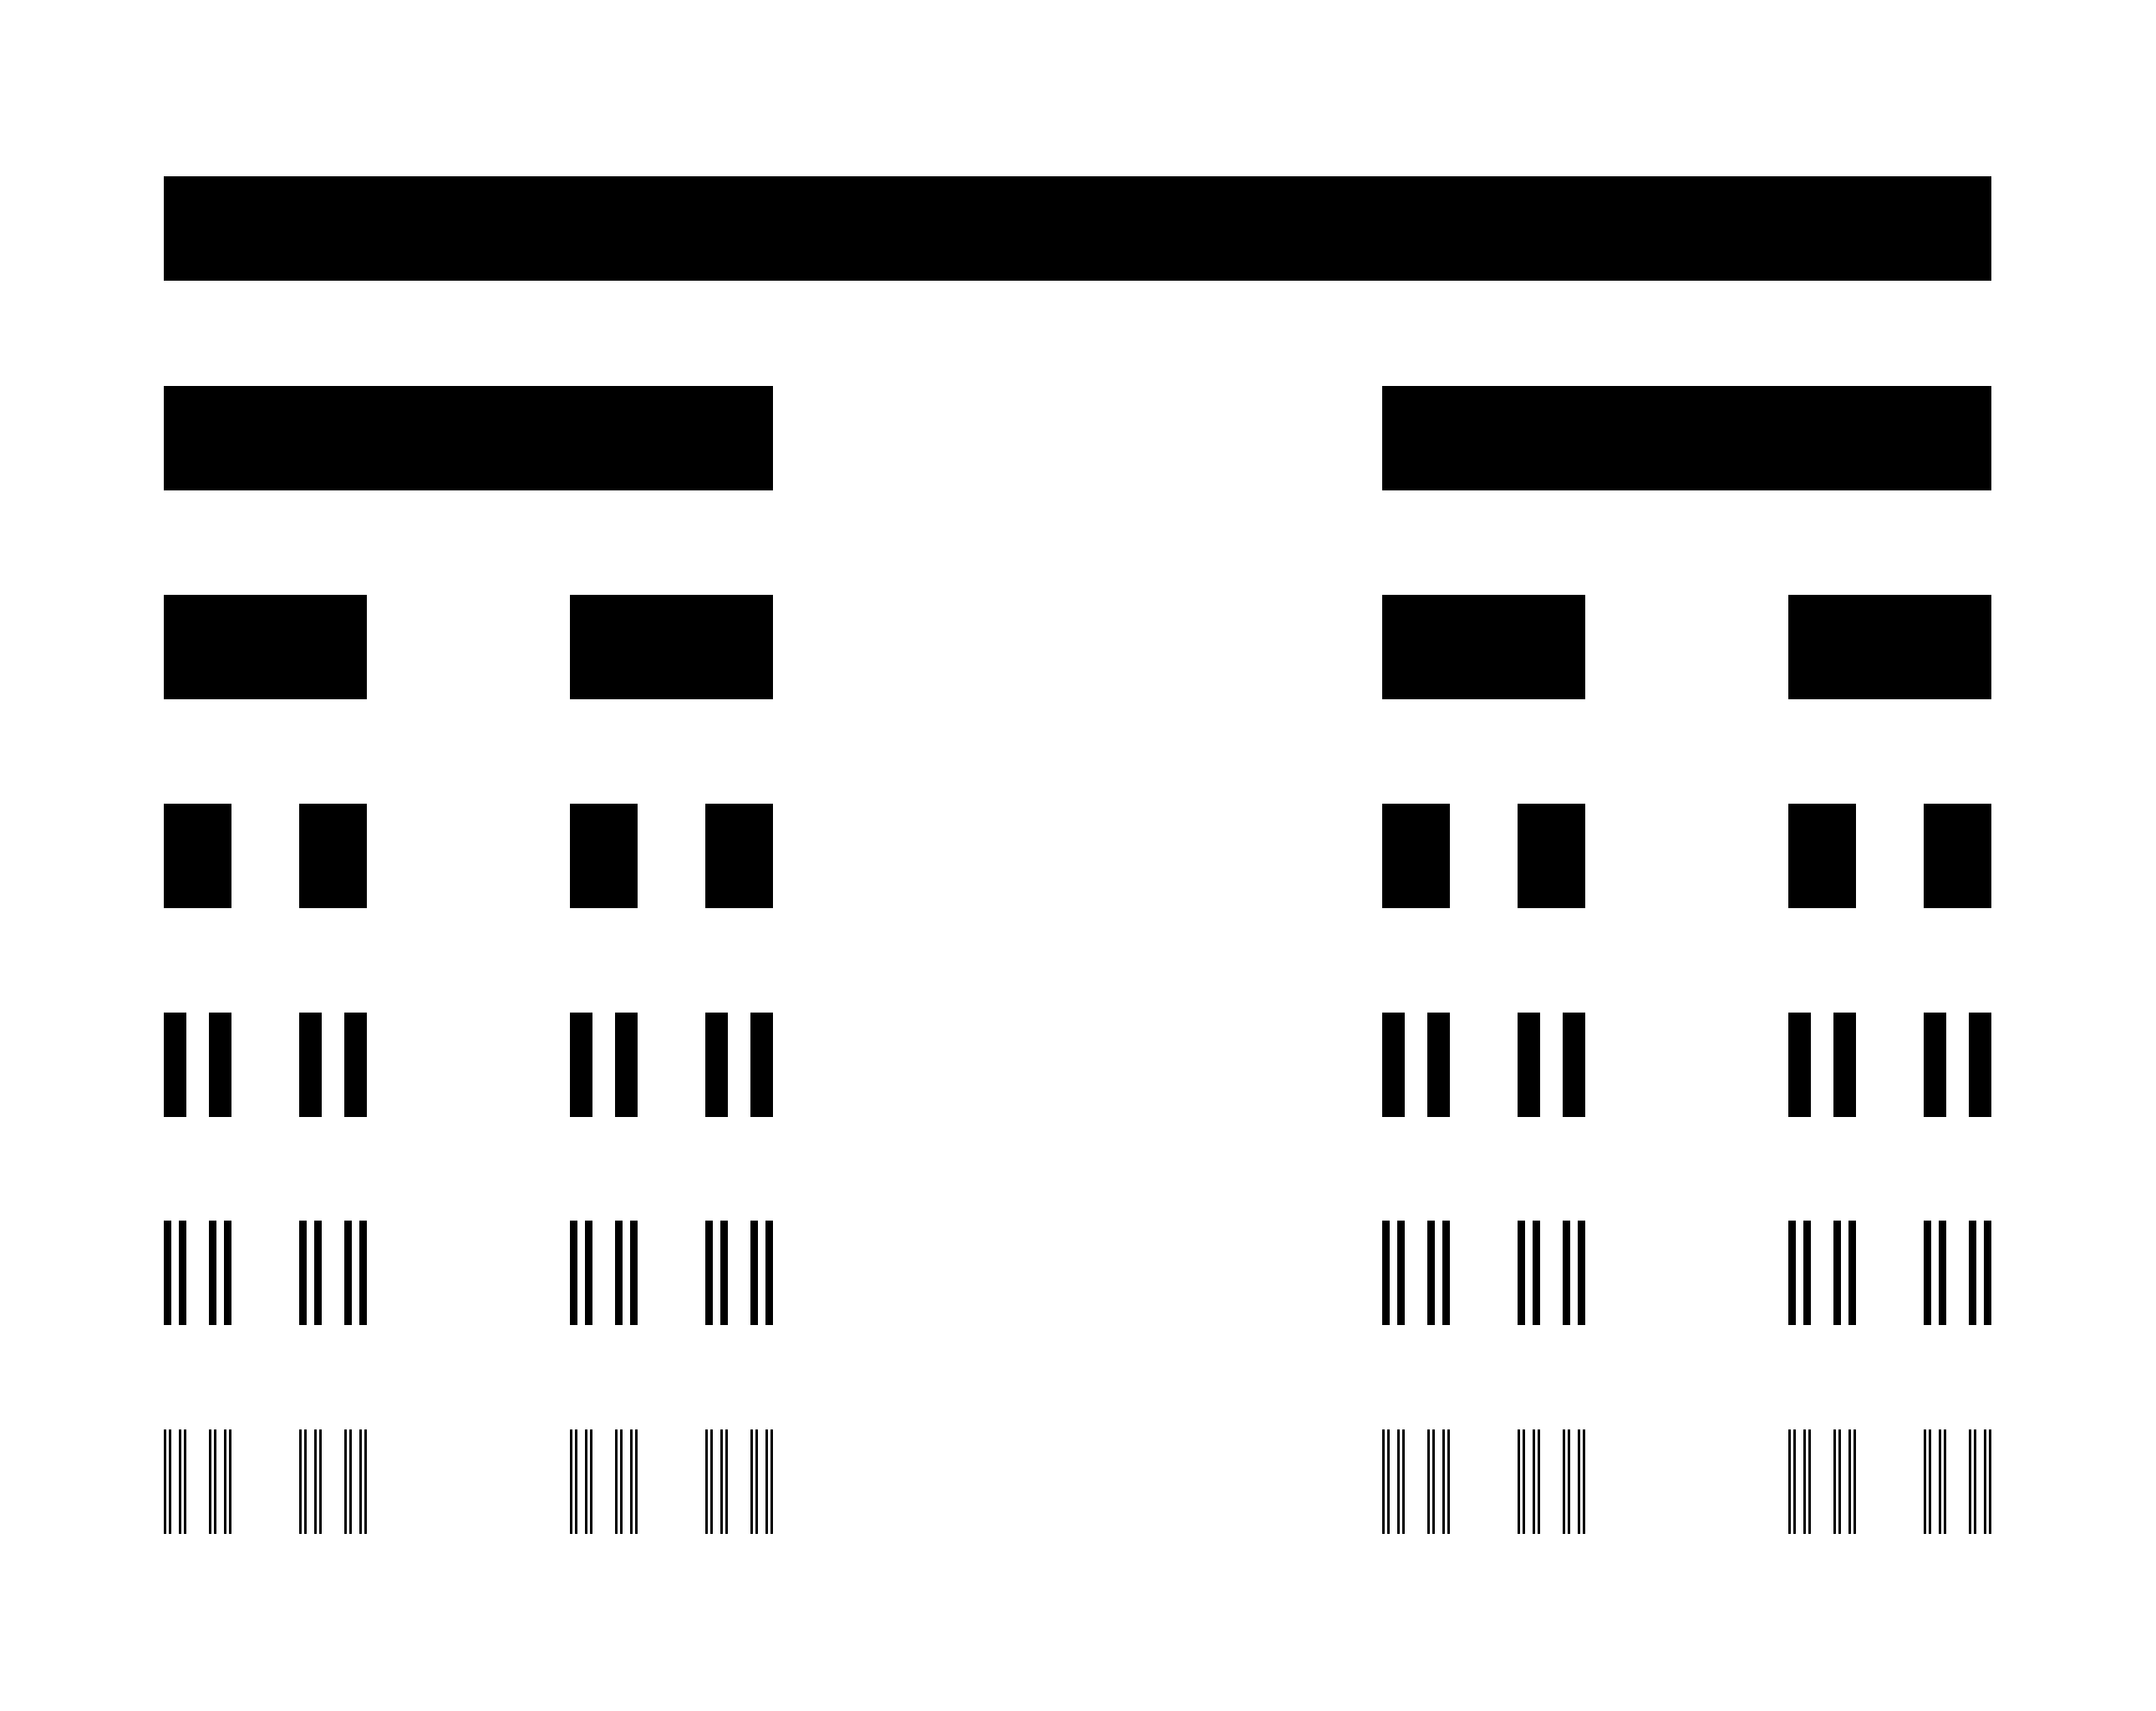
\includegraphics[scale=0.12]{cantor_set}}
\par\end{center}

\medskip{}

\textbf{הפונקציה המציינת של קבוצת קנטור:} \L{%
\[
\chi_{C}:[0,1]\to\{0,1\},\qquad\chi_{C}(x)=\begin{cases}
1 & x\in C\\
0 & x\notin C
\end{cases}
\]
}%

\medskip{}

\begin{center}
\L{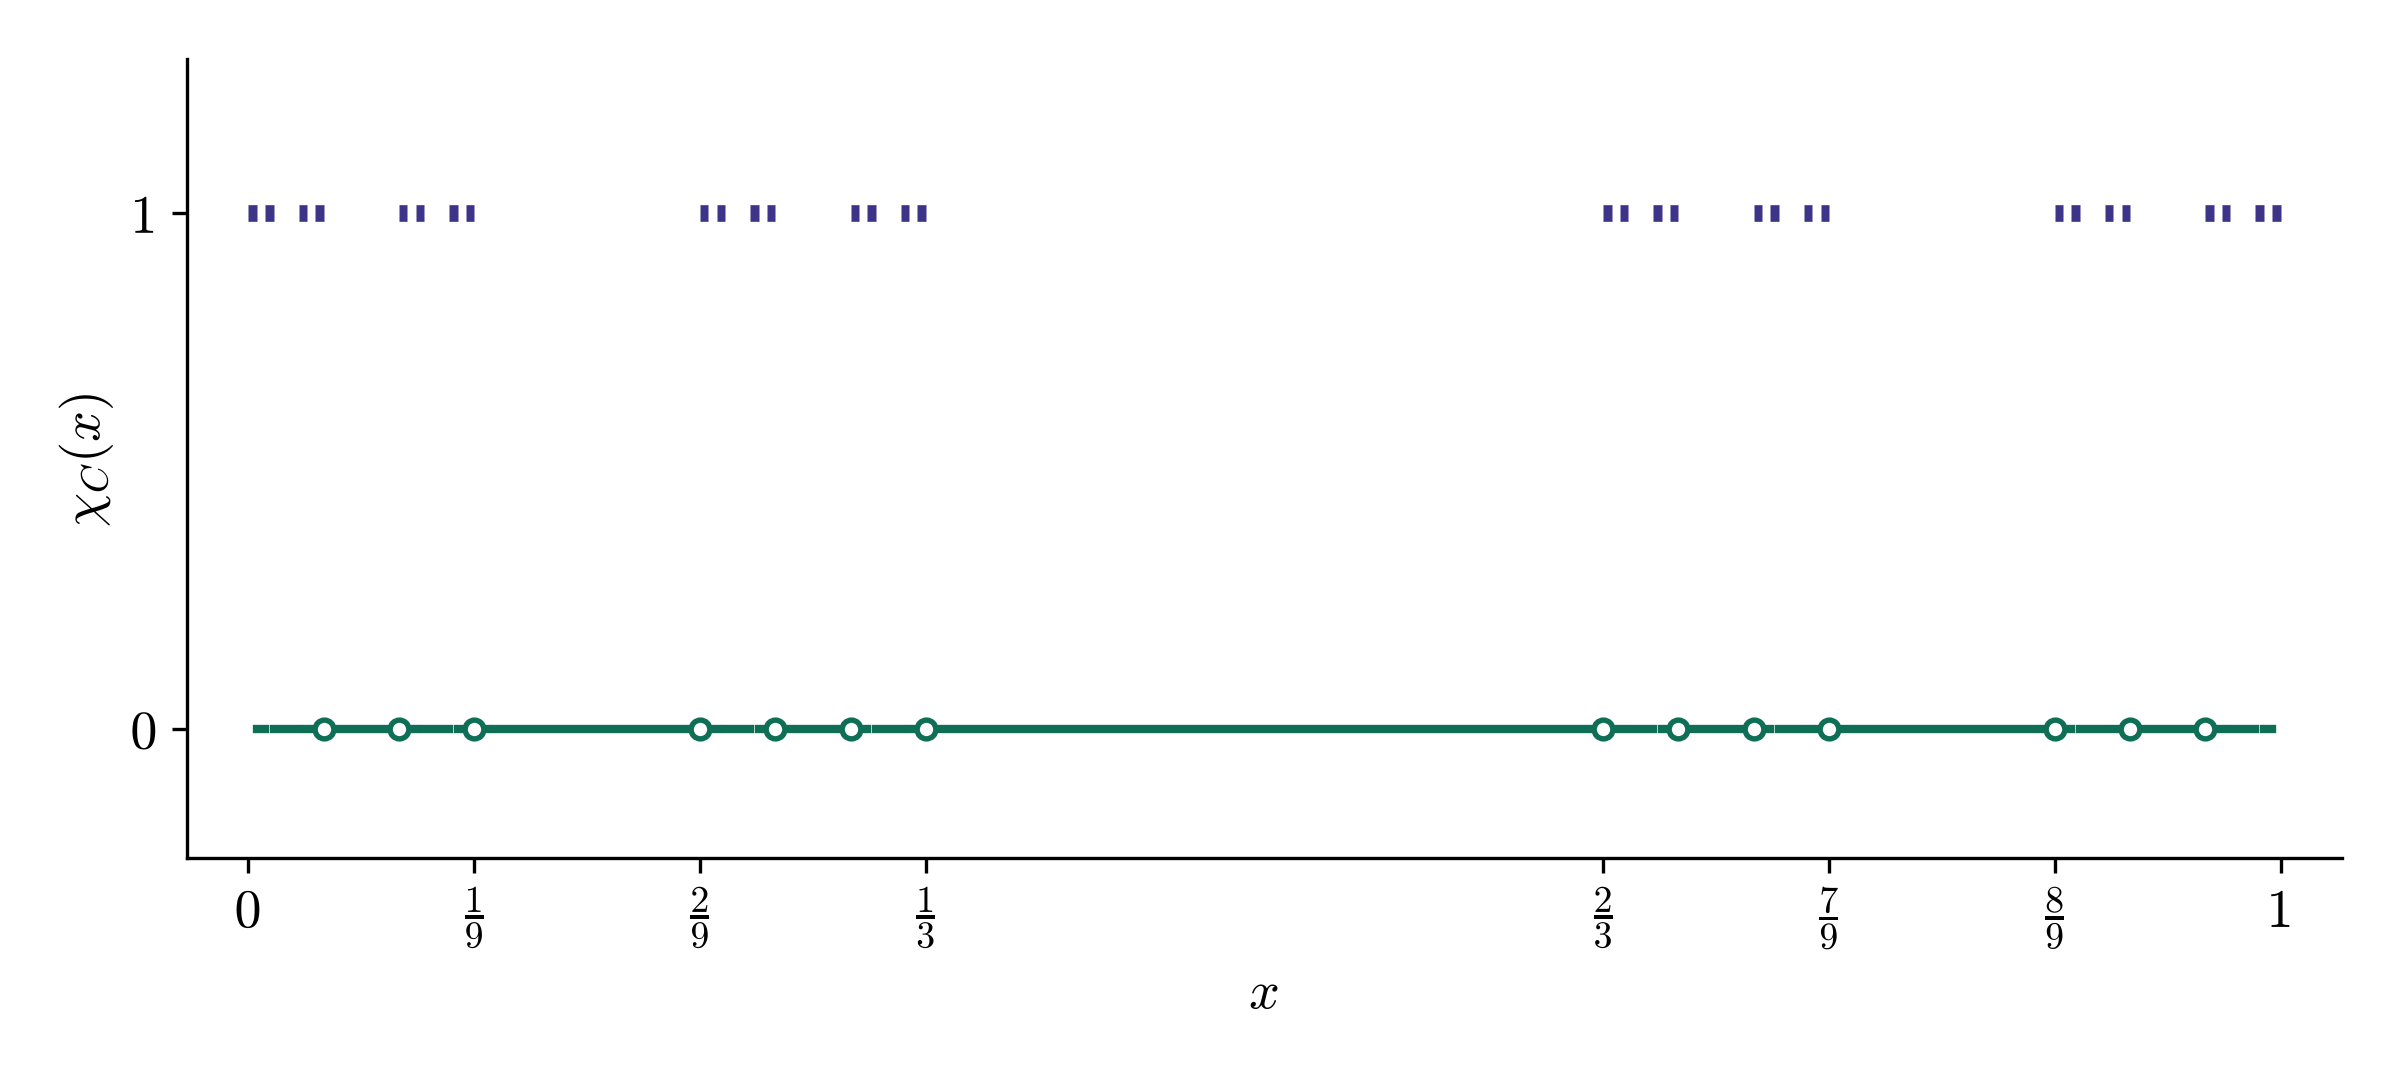
\includegraphics[scale=0.12]{cantor_func}}
\par\end{center}

\medskip{}

\part{העשרה - הרקע ההיסטורי, החשיבות של המשפט היסודי של החדו\textquotedblright א
וחזרה במילים על ההגדרות החשובות}

במשך זמן רב נחשבו שני מושגים במתמטיקה לבלתי קשורים זה לזה: השיפוע
של גרף, שהוא למעשה הנגזרת, והשטח הכלוא מתחת לגרף. 

המשפט היסודי של החדו\textquotedblright א מראה שיש ביניהם קשר הדוק.\\

בתחילת המאה ה-\L{$17$} הבחין האסטרונום הגרמני יוהאנס קפלר, על סמך
תצפיות מדויקות של מסלולי כוכבי הלכת, שהם נעים סביב השמש במסלולים אליפטיים. 

כעבור כמה עשורים פיתח פילוסוף של הטבע, אלכימאי בסתר, עמית בטריניטי
קולג' ופרופסור למתמטיקה באוניברסיטת קיימברידג' )בין שאר תארים מסקרנים(,
הלא הוא ניוטון, את תורת הכבידה שלו.

הוא ביקש לאשש אותה בעזרת ההבחנה של קפלר.

כדי להתמודד עם הבעיות הפיזיקליות שעמדו בפניו פיתח ניוטון את החשבון
הדיפרנציאלי והאינטגרלי.

במקביל אליו, באופן בלתי תלוי, פיתח אותו גם המתמטיקאי והפילוסוף הגרמני
גוטפריד וילהלם לייבניץ.

ניוטון )וגם לייבניץ( לא ביסס את התורה המתמטית שלו בנושא זה בצורה ריגורוזית
מספיק, ובגלל זה עלו אחר כך בעיות רבות, אף שמבחינה רעיונית היא הייתה
נכונה.

למשל, הוא השתמש במושג \emph{אינפיניטסימל}, גודל שונה מאפס אך קטן מכל
מספר חיובי, בלי להגדיר אותו בצורה מדויקת.

בנוסף, הוא הגדיר את האינטגרל כפעולה ההפוכה לגזירה, והגדרה זו שגויה
)בפרט, האינטגרל הלא מסוים שמתאר את קבוצת הפונ' הקדומות, והאינטגרל
המסוים, הם דברים שונים לחלוטין. יש פונ' אינטגרביליות שאין להן פונקציה
קדומה, ולהפך(.

עם זאת, ניוטון מצא את הקשר שמתואר במשפט היסודי.

נתבונן בפונקציה הצוברת \L{$\tilde{F}(x)=\int_{a}^{x}f(t)\,dt$}, שמתארת
את האינטגרל המסוים מ-\L{$a$} עד \L{$x$} כפונקציה של \L{$x$}. 

אם \L{$f$} רציפה )ולכן גם אינטגרבילית(, הפונקציה הצוברת היא פונקציה
קדומה של \L{$f$}.

ליתר דיוק, היא אחת מאינסוף הפונקציות הקדומות של \L{$f$}.
\begin{rem*}
זו אחת מני דוגמאות רבות הממחישות כיצד התיכון בעוולתו הרבה מלמד מתמטיקה
בצורה שגויה: בלימודים התיכוניים מבלבלים בין המושגים האלו ולא מבדילים
בין אינטגרל מסוים, פונ' צבירה, פונ' קדומה וכדומה.

נורא מכך, אטען שמתמטיקה תיכונית אינה שקולה למתמטיקה כלל )אולי יותר
לכיוון חשבון(, והנסיון המאולץ לכנות אותה ככה והלכה למעשה לשקר הוא
אחת הסיבות לסלידה הנפוצה ממתמטיקה בקרב תלמידי תיכון.
\end{rem*}
ניוטון השתמש במשפט הזה בתורת הכבידה שלו והגיע ממנה לתיאור של התנועה
האליפטית של כוכבי הלכת.

כך הוא קיבל בצורה מתמטית, מתוך התיאוריה שלו, את מה שקפלר הבחין בו
מתצפיות, וזה אישש מאוד את התיאוריה.

מחוקי ניוטון יחד עם המשפט היסודי נובע גם חוק שימור האנרגיה המכנית,
אף שהחוק עצמו נוסח במפורש רק במאה ה-\L{$19$}.

כל זה היה הבסיס להתפתחות המדעית שבאה אחריו.

רק יותר מ-\L{$150$} שנה אחרי ניוטון הוגדר האינטגרל בצורה מדויקת:
קושי הגדיר אותו ב-\L{$1823$} לפונקציות רציפות.

עברו עוד כשלושים שנה, כמעט מאתיים שנה מאז ניוטון, עד שרימן הכליל את
ההגדרה ב-\L{$1854$}.

לפי רימן, לוקחים קטע ומסתכלים על חלוקה כלשהי שלו.

בכל תת-קטע של החלוקה בוחרים נקודה שרירותית, מחשבים את אורך תת-הקטע
כפול ערך הפונקציה בנקודה שנבחרה, וסוכמים על פני כל תת-הקטעים. 

אם קיים מספר ממשי שהסכומים האלה שואפים אליו כאשר קוטר החלוקה שואף
לאפס, הפונקציה אינטגרבילית, והמספר הזה הוא האינטגרל.

הניסוח הזה אינו ריגורוזי לחלוטין.

קוטר החלוקה הוא האורך המקסימלי של תת-קטע בחלוקה, ולכן הוא פונקציה
שמוגדרת על חלוקות, וחלוקה היא קבוצה סופית של נקודות. 

לכן הביטוי \emph{גבול כאשר הקוטר שואף לאפס} אינו גבול רגיל של פונקציה
ממשית. 

הניסוח המדויק הוא: קיים \L{$I$} ממשי כך שלכל \L{$\varepsilon>0$}
קיימת \L{$\delta>0$}, כך שלכל חלוקה \L{$P$} שקוטרה קטן מ-\L{$\delta$}
ולכל בחירה של נקודות ביניים \L{$P^{*}$} מתקיים \L{$\left|S\left(f,P,P^{*}\right)-I\right|<\varepsilon$}. 

לכל מרחק קטן כרצוננו, אם נעדן את החלוקה מספיק באופן מתאים )כך שהקוטר
שלה יקטן(, סכום ערכי הפונקציה בנקודות השרירותיות כפול אורכי תת-הקטעים
יהיה קרוב ל-\L{$I$} עד כדי אותו מרחק. 

הדלתא קובעת כמה עדינה צריכה להיות החלוקה, כלומר כמה קטן צריך להיות
הקוטר שלה.

זמן קצר אחרי רימן הציע דארבו דרך נוספת לאפיין את האינטגרביליות לפי
רימן, שאולי קלה יותר להבנה.

תהי \L{$f$} חסומה בקטע סגור, ונסתכל על חלוקה כלשהי שלו. 

בכל תת-קטע לוקחים את הסופרמום של ערכי הפונקציה, כופלים באורך תת-הקטע
וסוכמים. 

זהו סכום דארבו העליון, והאינפימום של הסכומים האלה על פני כל החלוקות
האפשריות הוא האינטגרל העליון. 

באופן דומה, לוקחים בכל תת-קטע את האינפימום של ערכי הפונקציה, כופלים
באורך וסוכמים.

זהו סכום דארבו התחתון, והסופרמום של הסכומים האלה על פני כל החלוקות
הוא האינטגרל התחתון.

אם שני המספרים הממשיים האלה שווים, הפונקציה אינטגרבילית לפי דארבו,
והמספר המשותף הוא האינטגרל שלה. 

אינטגרביליות לפי דארבו שקולה לאינטגרביליות לפי רימן.

דארבו עובד עם הסופרמום והאינפימום של הפונקציה בכל תת-קטע, כלומר עם
התנודות שלה, ואילו רימן עובד עם נקודות שרירותיות בכל תת-קטע.\\

\begin{center}
\L{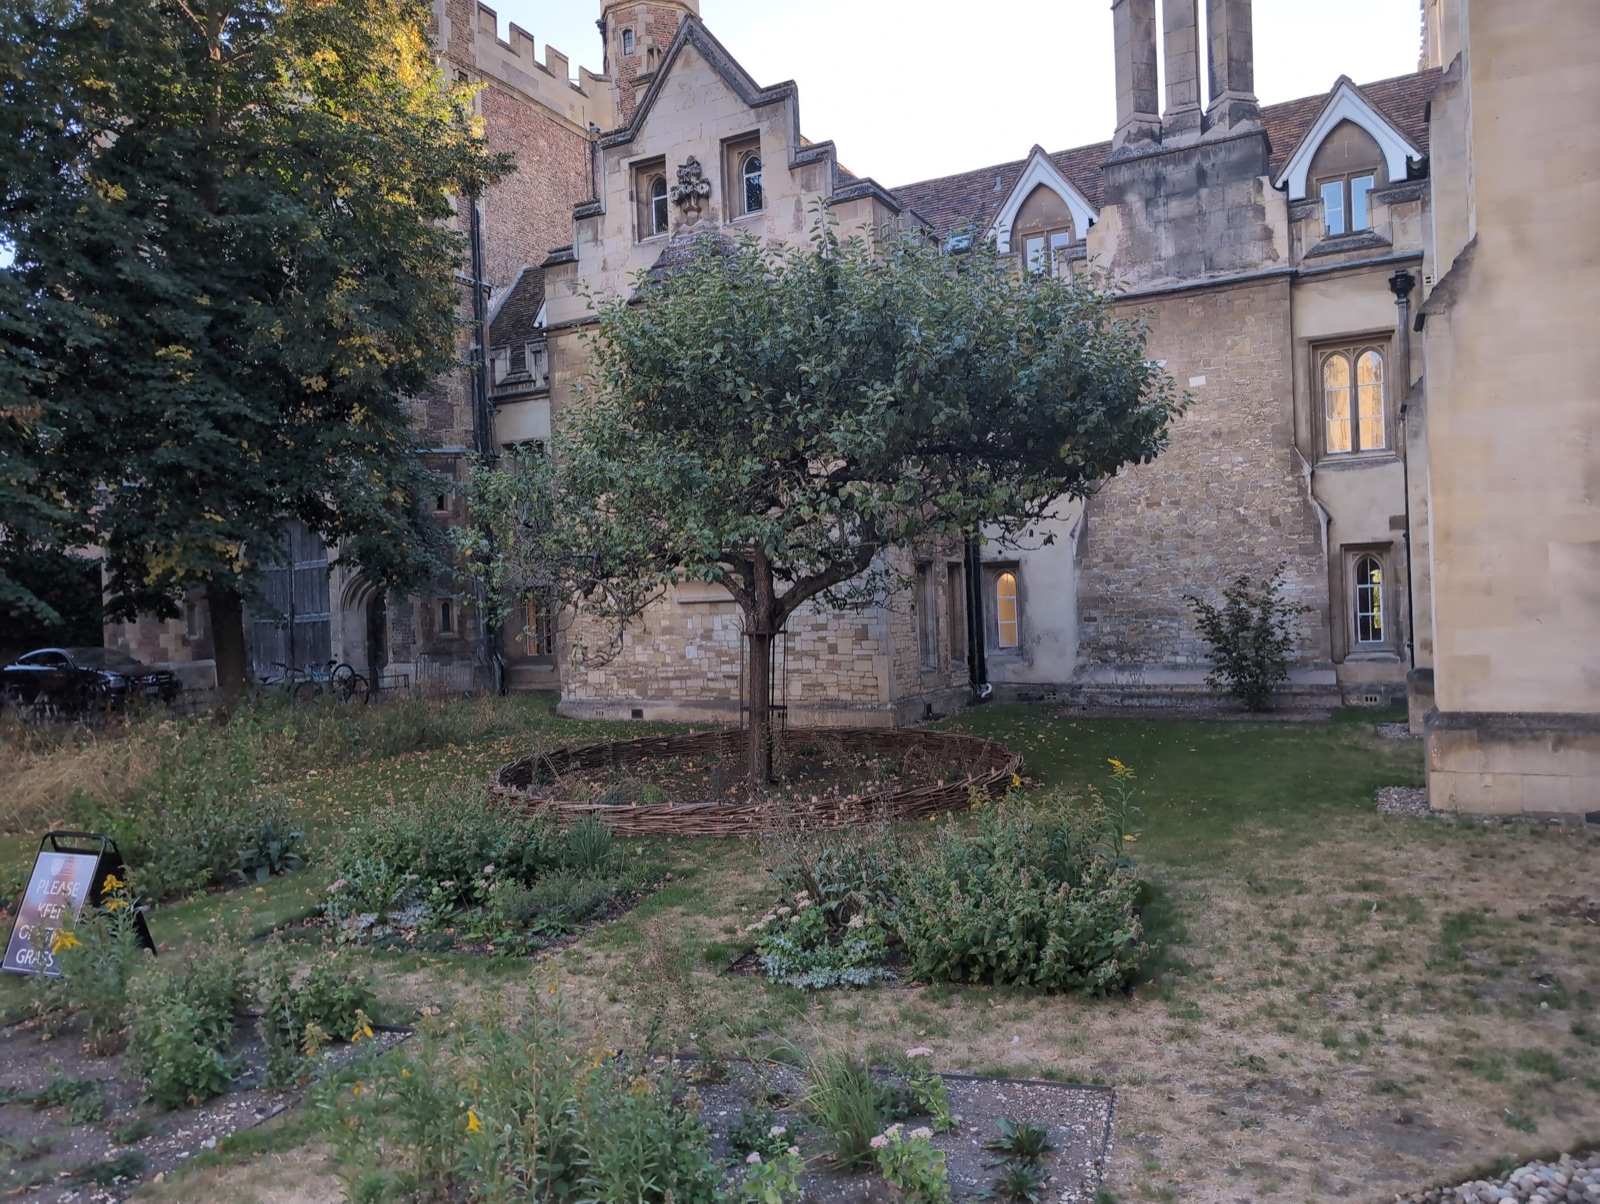
\includegraphics[scale=0.12]{cambridgetree}}
\par\end{center}

בתמונה: עץ התפוח של ניוטון ששיבטו מול טריניטי קולג'\\

הגיפים של סכומי דארבו: \L{IkamusumeFan}, ויקישיתוף, רישיון \L{CC BY-SA
3.0}
\end{document}
